\documentclass[12pt]{article}
\usepackage[utf8]{inputenc}
\usepackage[left=2.5cm, right=2.5cm, top=2.0cm]{geometry}
\usepackage{sectsty}
\usepackage{graphicx}
\usepackage{amsmath}
\usepackage{amssymb}
\usepackage{undertilde}
\usepackage{kbordermatrix}
\usepackage{listings}
\usepackage{ulem}
\usepackage{soul}
% \usepackage{tikz}
% \usepackage{pgfplots}
% \pgfplotsset{compat=1.16} 
\usepackage{siunitx}
\usepackage{pythonhighlight}
\usepackage{caption}
\usepackage{float}
\usepackage{url}
\usepackage{enumitem}
\usepackage{bm}
\usepackage{empheq}
\usepackage{tcolorbox}
\usepackage{framed}
\usepackage{xparse}
\usepackage{algorithm, algorithmic}
% \usepackage{algorithmic}
\usepackage{booktabs}
\usepackage{tabularx}
% ref packages
\usepackage{nameref}
% folowing  must be in this order
\usepackage{varioref}
\usepackage{hyperref}
\usepackage{cleveref}
\usepackage{mathtools}
\DeclareMathOperator*{\argmax}{arg\,max}
% \usepackage[shortlabels]{enumitem}
\tcbuselibrary{breakable}
\allowdisplaybreaks


%  ---------------------- COMMANDS ---------------------------
% Double underline
\def\dunderline#1{\underline{\underline{#1}}}

% Shorten nonumber command
\def\nnb{\nonumber}

% Shorten boldsymbol command
\def\bs#1{\boldsymbol{#1}}

% Algorithmic newline
\def\algonewline{\STATE{ }}

% Eigenvectors of
\def\eigvecof{\text{eigenvectors of }}

% Eigenvalues of 
\def\eigvalof{\text{eigenvalues of }}

% Enclose in square brackets
\newcommand{\enclb}[1]{\left[#1\right]}
% Enclose in parenthesis
\newcommand{\enclp}[1]{\left(#1\right)}
% Enclose in curly brackets
\newcommand{\enclc}[1]{\left\{#1\right\}}

% Annotate first argument, text in second argument
\newcommand{\overtext}[2]{\overbrace{#1}^{\mathclap{\text{#2}}}}
\newcommand{\undertext}[2]{\underbrace{#1}_{\mathclap{\text{#2}}}}

% Normalization constant in multivariate normal
\newcommand{\mvnconst}[1]{\frac{1}{(2\pi)^{d/2} |#1|^{1/2}}}

% Exponential factor in multivariate normal
\newcommand{\mvnexpo}[3][x]{\exp \left[  -{\frac{1}{2}} (#1 - #2)^T #3^{-1} (#1 - #2) \right]}

% Multivariate normal
\newcommand{\mvn}[3][x]{\mvnconst{#3} \mvnexpo[#1]{#2}{#3}}

% For numbering in align* environment
\newcommand{\numberthis}{\addtocounter{equation}{1}\tag{\theequation}}

%  Sum notation w/ limits as argument and index as option
\newcommand{\sumlim}[3][i]{\sum\limits_{#1=#2}^{#3}}

%  Product notation w/ limits as argument and index as option
\newcommand{\prodlim}[3][i]{\prod\limits_{#1=#2}^{#3}}

%  Sum notation with only information beneath
\newcommand{\sumnolim}[1]{\sum\limits_{#1}}

%  Integral notation w/ limits as argument and index as option
\newcommand{\intlim}[2]{\int\limits_{#1}^{#2}}

%  Integral over whole domain notation, no args
\newcommand{\intinf}{\int\limits_{-\infty}^{\infty}}

%  Partial derivative notation, arg1: numerator, arg2: denominator
\newcommand{\pfrac}[3][ ]{\frac{\partial^{#1} #2}{\partial #3^{#1}}}

%  Derivative notation, arg1: numerator, arg2: denominator
\newcommand{\dvfrac}[3][ ]{\frac{\text{d}^{#1} #2}{\text{d} #3^{#1}}}

% When doing Gauss-Jordan, create arrow showing operations
\newcommand{\ro}[1]{\xrightarrow{\mathmakebox[\rowidth]{#1}}}

% ----------------------INVIRONMENTS---------------------------
% Item list with title
\newenvironment{titlemize}[1]{%
  \paragraph{#1}
  \begin{itemize}}
  {\end{itemize}}

  % Enum list with title
\newenvironment{titleenum}[1]{%
  \paragraph{#1}
  \begin{enumerate}}
  {\end{enumerate}}

  % Augmented matrix (matrix with vertical line)
\newenvironment{sysmatrix}[1]
  {\left(\begin{array}{@{}#1@{}}}
  {\end{array}\right)}

 % Make matrices with more spacing
\makeatletter
\renewcommand*\env@matrix[1][\arraystretch]{%
  \edef\arraystretch{#1}%
  \hskip -\arraycolsep
  \let\@ifnextchar\new@ifnextchar
  \array{*\c@MaxMatrixCols c}}
\makeatother

% \renewcommand*{\arraystretch}{1.5}

\newlength{\rowidth}% row operation width
\AtBeginDocument{\setlength{\rowidth}{3em}}

\floatname{algorithm}{Algorithm}
\renewcommand{\algorithmicrequire}{\textbf{Input:}}
\renewcommand{\algorithmicensure}{\textbf{Output:}}

\begin{document}
\title{\textbf{INF367A Exercise 9}}
\author{Naphat Amundsen}
\maketitle
\sectionfont{\fontsize{14}{15}\selectfont}
\subsectionfont{\fontsize{12}{15}\selectfont}
\subsubsectionfont{\fontsize{12}{15}\selectfont}
\graphicspath{ {./images/} }

\ifx
\begin{figure}[H]
	\centering
	\includegraphics[scale=0.8]{Figure_2}
	\caption{Insert caption here}
\end{figure}
\fi

\section*{Introduction}
    This exercise is about sampling methods
    \vspace{5mm}
    \begin{tcolorbox}[breakable]
        \textbf{Context:} Earlier, we have performed Bayesian linear regression assuming that the noise precision $\beta$ is known. Let us now formulate a full Bayesian linear regression model by placing a prior on $\beta$. 

        Assume that we have observed $n$ pairs $(x_i, y_i)$ where $x_i$ are the feature values and $y_i$ is the label. Let $w \in \mathbb{R}^d$ be our regression weights. The likelihood is 
        \begin{align*}
            P(y|x,w,\beta) = \prodlim{1}{n}N(y_i|w^Tx_i, \beta^{-1}).
        \end{align*}
        As earlier, we place Gaussian prior on the regression weights:
        \begin{align*}
            P(w) = N(w|0, \alpha^{-1}I)
        \end{align*}
        where $\alpha$ (prior precision) is a user-defined hyperparameter. For $\beta$, we use a Gamma prior 
        \begin{align*}
            P(\beta) = \operatorname{Gamma}(\beta|a_0, b_0)
        \end{align*}
        where $a_0$ and $b_0$ are user-defined hyperparameters. \\ 

        The goal is to compute the posterior
        \begin{align*}
            P(w,\beta|x,y)
        \end{align*}
        This distribution does not have a closed-form solution and therefore we use sampling to approximate the posterior. 
    \end{tcolorbox}

\section{Gibbs sampling}
    \subsection{Derive conditional distributions}
        \begin{tcolorbox}
            Derive a Gibbs sampler for the above model. That is, derive the full conditional distributions $P(w|x,y,\beta)$ and $P(\beta|x,y,w).$\\
            Hint: When deriving the conditional distribution for $w$ or $\beta$, you can drop all terms that do not depend on $w$ or $\beta$, respectively. Note that both distributions involve conjugate priors.  
        \end{tcolorbox}
        % \newcommand{\mvnexpol}[2]{\exp \left[  -{\frac{1}{2}} #1^T #2 #1 \right]}
        \newcommand{\mvnexpol}[2]{e^{-{\frac{1}{2}} #1^T #2 #1}}
        \newcommand{\opGamma}[0]{\operatorname{Gamma}}

        \subsubsection*{Case for $w$}
            Let $a=a_0,\ b=b_0$
            \begin{align}
                P(w|y, x, \beta) &\propto P(\beta) P(w) P(y|x,w,\beta)\\
                &= \opGamma(\beta|a, b) \cdot N(w|0,\alpha I) \cdot \prodlim{1}{n} N(y_i - w^T x_i) \\
                &= \frac{1}{\Gamma(a)}b^{a}\beta^{a-1}e^{-b\beta}\mvnexpol{w}{\alpha I} \prodlim{1}{n} \mvnexpol{(y_i - w^T x_i)}{\beta} \\ 
                &\propto \exp\enclb{-\frac{1}{2}w^T\alpha Iw + \sumlim{1}{n}-\frac{1}{2}(y_i-w^Tx_i)^T\beta(y_i-w^Tx_i)}
            \end{align}

            Logarithm the thing to make math doable
            \begin{align}
                \Rightarrow \ln P(w|y, x, \beta) &= \ln \enclp{\exp\enclb{-\frac{1}{2}w^T\alpha Iw + \sumlim{1}{n}-\frac{1}{2}(y_i-w^Tx_i)^T\beta(y_i-w^Tx_i)}} \\ 
                &= -\frac{1}{2} w^T \alpha I w -\frac{1}{2} \sumlim{1}{n} (y_i - w^T x_i)^T \beta (y_i - w^T x_i) \\ 
                &= -\frac{1}{2} \left[ w^T \alpha I w + \sumlim{1}{n} (y_i - w^T x_i)^T \beta (y_i - w^T x_i) \right] 
            \end{align}
            Now want to write the thing in quadratic form:
            \begin{align}
                \frac{1}{2} \theta^T A \theta + b^T \theta
            \end{align}
            Let $w^T x_i = p$ (don't want to use $\hat{y_i}$ since it confuses me when there are a lot of $y_i$ symbols as well)

            \begin{align}
                &= -\frac{1}{2} \left[ w^T \alpha I w + \sumlim{1}{n} (y_i - p_i)^T \beta (y_i - p_i) \right] \\
                &= -\frac{1}{2} \left[ w^T \alpha I w + \sumlim{1}{n} y_i^T \beta y_i - y_i^T \beta p_i - p_i^T \beta y_i + p_i^T \beta p_i \right] \\
                &\propto -\frac{1}{2} \left[ w^T \alpha I w + \sumlim{1}{n} \overtext{- y_i^T \beta p_i - p_i^T \beta y_i + p_i^T \beta p_i}{$\beta$ is scalar} \right] \\
                &= -\frac{1}{2} \Big[ w^T \alpha I w + \sumlim{1}{n} - y_i^T \beta p_i - y_i^T \beta p_i + p_i^T \beta p_i \Big] \\
                &= -\frac{1}{2} \Big[ w^T \alpha I w + \sumlim{1}{n} - 2 y_i^T \beta p_i + p_i^T \beta p_i \Big] \\
                &= -\frac{1}{2} \enclb{w^T \alpha I w + \sumlim{1}{n} - 2 y_i^T \beta w^Tx_i + \beta w^T x_i x_i^T w} \\
                &= -\frac{1}{2} \enclb{w^T \alpha I w - 2 \sumlim{1}{n} y_i^T \beta x_i^Tw + \sumlim{1}{n} \beta w^T x_i x_i^T w} \\
                &= -\frac{1}{2} \enclb{w^T \enclp{\alpha I + \beta \sumlim{1}{n} x_ix_i^T} w - 2 \enclp{\beta \sumlim{1}{n} y_i^T x_i^T} w} \\ 
                &= -\frac{1}{2} w^T \enclp{\alpha I + \beta \sumlim{1}{n} x_ix_i^T} w + \enclp{\beta \sumlim{1}{n} y_i^T x_i^T} w
            \end{align}
            Now it is in quadratic form yo, let 
            \begin{align}
                A = \enclp{\alpha I + \beta \sumlim{1}{n} x_i x_i^T}, \quad b = \enclp{\beta \sumlim{1}{n} y_i x_i} 
            \end{align}
            Then by completing the square, we obtain the parameters $S$ (variance), $m$ (mean) for a Gaussian (see lecture slides).
            \begin{align}
            S &= A^{-1} = \enclp{\alpha I + \beta \sumlim{1}{n} x_i x_i^T}^{-1} \label{eq:S}\\ 
            m &= A^{-1} b = \beta S \sumlim{1}{n} y_i x_i \label{eq:m}\\ 
            &\dunderline{\Rightarrow P(w|y,x,\beta) = \mathcal{N}(w|m,S)}
            \end{align}

        \subsubsection*{Case for $\beta$}
            Let $a=a_0,\ b=b_0$
            \begin{align}
                P(b|x, y, w) &\propto P(\beta) P(w) P(y|x,w,\beta)\\
                &= \opGamma(\beta|a, b) \cdot N(w|0,\alpha I) \cdot \prodlim{1}{n} N(y_i - w^T x_i) \\
                &= \frac{1}{\Gamma(a)}b^{a}\beta^{a-1}e^{-b\beta}\mvnexpol{w}{\alpha I} \prodlim{1}{n} \mvnexpol{(y_i - w^T x_i)}{\beta} \\ 
                &\propto \beta^{a-1}e^{-b\beta} \prodlim{1}{n} \mvnexpol{(y_i - w^T x_i)}{\beta} \\ 
                &= \beta^{a-1} \exp\enclb{-b\beta + \sumlim{1}{n} -\frac{1}{2}(y_i-w^Tx_i)^T\beta(y_i-w^Tx_i)} \\ 
                &= \beta^{a-1} \exp\enclb{-\beta\enclp{b + \frac{1}{2} \sumlim{1}{n} (y_i-w^Tx_i)^T(y_i-w^Tx_i)}} \\
                &\propto \dunderline{\opGamma(a, b+\frac{1}{2} \sumlim{1}{n} (y_i-w^Tx)^T(y_i-w^Tx_i))}
            \end{align}

    \subsection{Implement the Gibbs sampler} \label{sec:fuck}
        \begin{tcolorbox}[breakable]
            Implement the Gibbs sampler. Download the data new\_york\_bicycles.csv. The first column is the number of daily riders on Brooklyn Bridge $(x)$ and the second column is the number of daily riders on Manhattan Bridge $(y)$. Use your Gibbs sampler to learn a simple linear model (intercept and slope) for this data. 
            
            \vspace{3mm}
            Compute the logarithm of the joint probability of the parameter values (which is proportional to the posterior).
            \begin{align*}
                \log P(y,x,w^{t},\beta^{t}) = \log P(\beta^{t}) + \log P(w^{t}) + \sumlim{1}{n} \log P(y_i|x_i,w^{(t)},(\beta^{(t)})^{-1})
            \end{align*}

            after each iteration. Plot a trace plot of these values (x-axis is the iteration number). What can you say about the convergence based on this plot? Plot trace plots for the parameter values $w_0$ , $w_1$ and $\beta$. What can you say about convergence and mixing based on these plots. Plot the marginal distributions of the parameters $w_0$ , $w 1$ and $\beta$. Remember to exclude burn-in. 

            \vspace{3mm}
            Hint: Remember that $\operatorname{Gamma}(a,b)$ is gamma(a=a, scale=1/b) in Scipy. 
            
            Hint: You want sample thousands of samples. Typically, burn-in is about half of the samples.
        \end{tcolorbox}
        \pagebreak
        \subsubsection*{Idea}
            \begin{enumerate}
                \item Initialize values for $w_0^0, w_1^0, \beta$
                \item For index $t$ in $n$ iterations do:
                \begin{enumerate}[label*={\arabic*.}]
                    \item Sample $(w_0^{t+1}, w_1^{t+1})$ from $\mathcal{N} \enclp{w^t|m^t, S^t}$ ($m$ and $S$ are defined in (\ref{eq:m}) and (\ref{eq:S}))
                    \item Sample $\beta^{t+1}$ from $\opGamma \enclp{a, b+\frac{1}{2} \sumlim{1}{n} (y_i-{w^t}^Tx)^T (y_i-{w^t}^Tx_i)}$
                \end{enumerate}
                \item Plot the posterior (or something proportional to it) for each iteration.
                \item Plot the parameters for each iteration. 
            \end{enumerate}
        
        \begin{figure}[H]
            \centering
            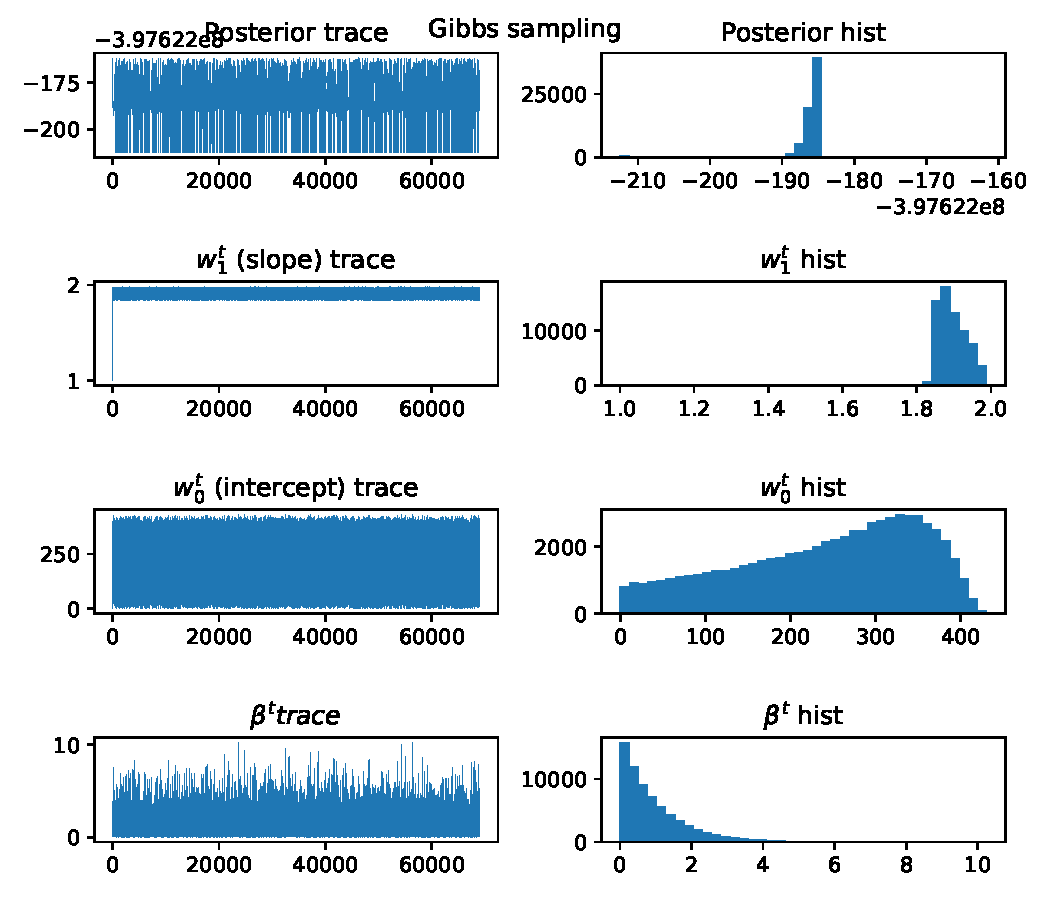
\includegraphics[width=0.8\textwidth]{gibbs.pdf}
            \caption{Just looking at the trace plots does not give me very much, but the histograms looks nice and looks reasonable.}
        \end{figure}
        \begin{figure}[H]
            \centering
            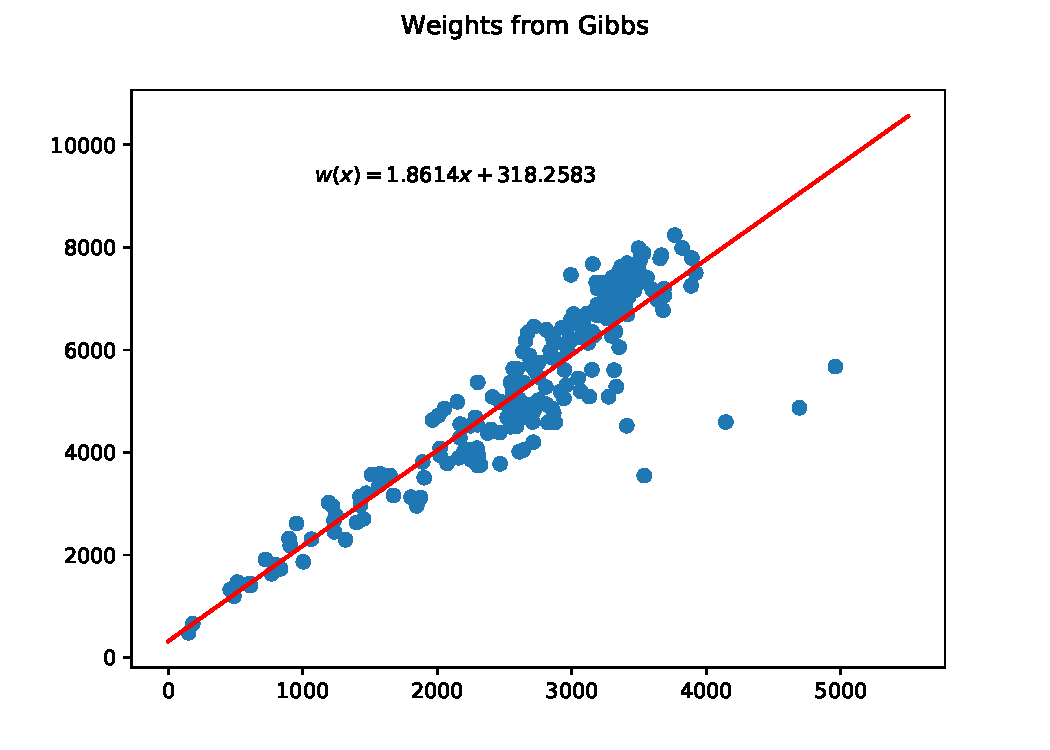
\includegraphics[width=0.8\textwidth]{regline_gibbs.pdf}
            \caption{Taking the argmax of the regression weight histograms gives a reasonable trendline.}
        \end{figure}


\section{Metropolis(-Hastings) Algorithm}
    \begin{tcolorbox}
        Derive a Metropolis(-Hastings) algorithm. That is, come up with a proposal distribution $q(w^*,\beta^*|w,\beta).$ You should probably add a parameter or two controlling the "step-size", that is, how far from the current values can the proposed values be.
    \end{tcolorbox}
    Use multivariate normal distribution with diagonal covariance matrix since I like it (and it is radially symmetric when there is no covariance, which is nice). Algorithm is then:
    \begin{enumerate}
        \item Initialize $\theta = (w_0^0, w_1^0, \beta^0)$
        \item for index $t$ in iterations:
        \begin{enumerate}[label*={\arabic*.}]
            \item Sample $\theta^*$ from $\mathcal{N}(\theta^{t-1}, \Sigma)$
            \item Let $A = \min \enclc{1, \frac{P(\theta^*|D)}{P(\theta^{t-1}|D)}}$
            \item Sample $u \sim \operatorname{Uniform(0,1)}$
            \item If $u < A$, set $\theta^t = \theta^*$, else $\theta^t = \theta^{t-1}$  
        \end{enumerate}
    \end{enumerate}

    \begin{tcolorbox}
        Implement the Metropolis-Hastings algorithm and do the same steps as in section \ref{sec:fuck}. In addition, keep track of the proportion of proposal that were actually accepted.
        
        \vspace{3mm}
        Hint: To avoid numerical problems in computing the acceptance ratio,
        one can use the following formula:
        $$\frac{P(k^*)}{P(k)}=e^{\log P(k^*)-\log P(k)}.$$

        Note that here you need the logarithm of the joint probability which you implemented already in task 2.
    \end{tcolorbox}
    \begin{figure}[H]
        \centering
        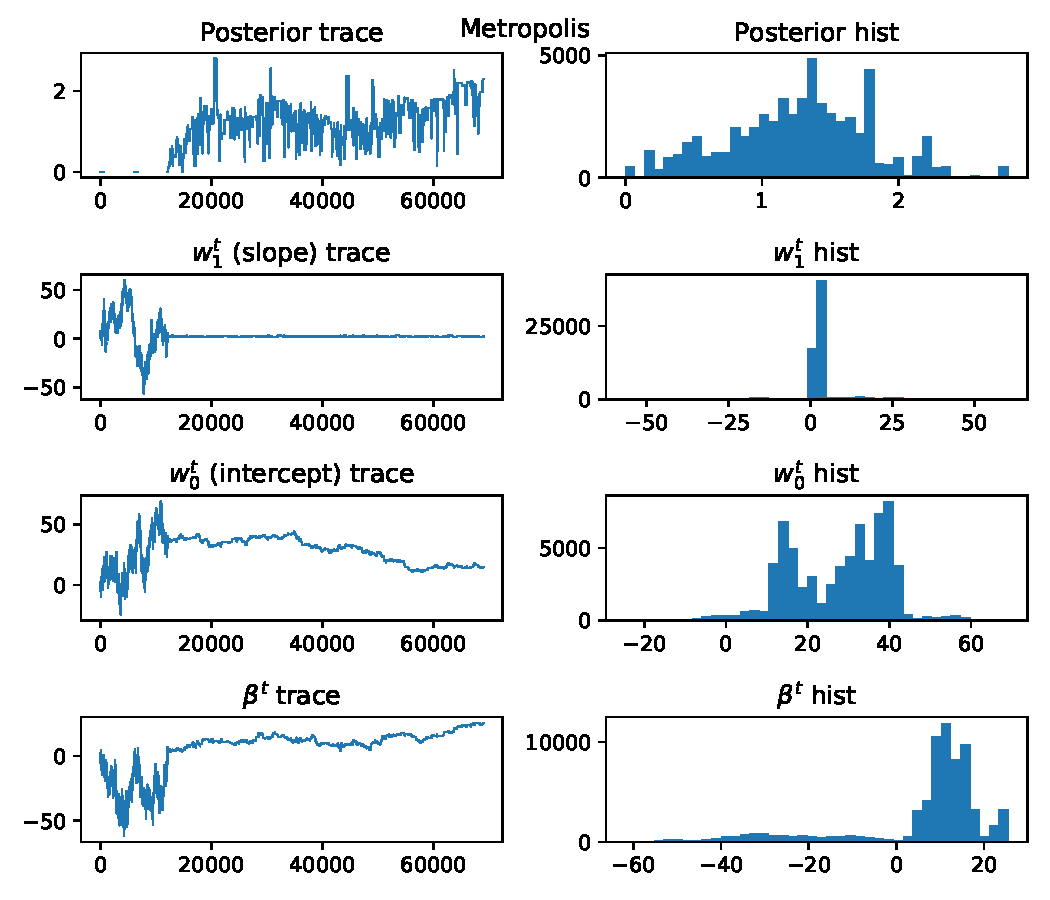
\includegraphics[width=0.8\textwidth]{metropolis2.pdf}
        \caption{The burnout time seems to end at 20000 iterations according to my eyes. Afterwards we see that the parameter values stay relatively flat opposed to movement during the burnout. The histograms aren't as nice as Gibbs though, but they include the burnout values.}        
    \end{figure}
    \begin{figure}[H]
        \centering
        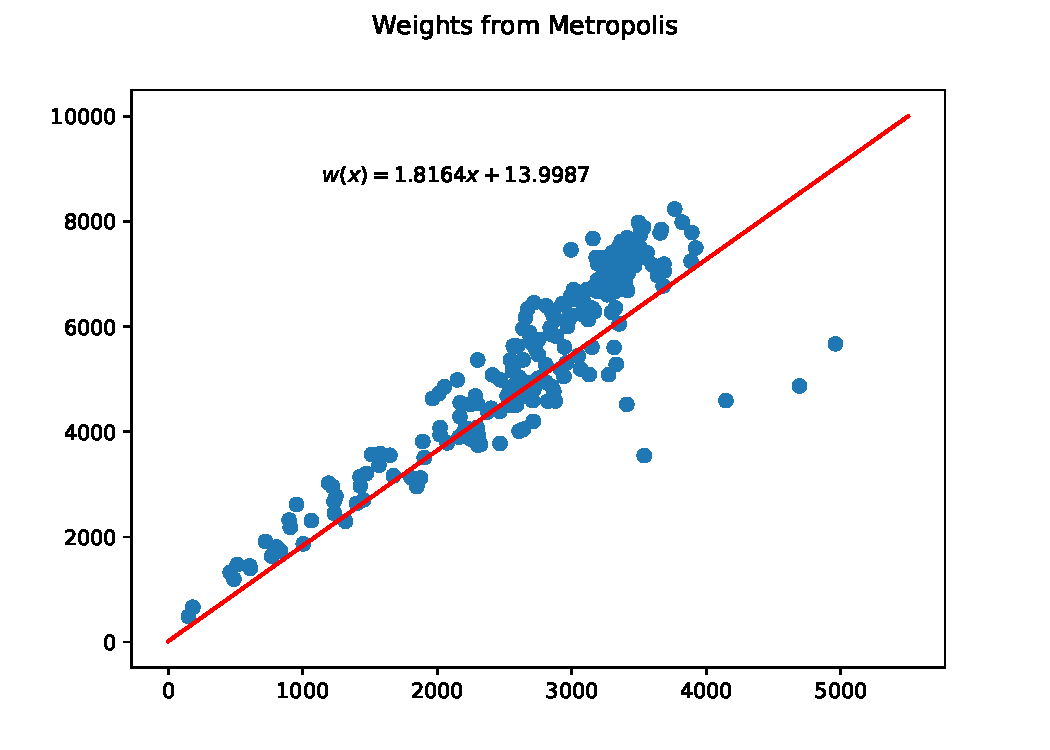
\includegraphics[width=0.8\textwidth]{regline_metropolis.pdf}
        \caption{After cutting the first 20 000 samples (the burnout), then doing argmax on the histograms of the samples linear regression parameters resulted in a reasonable regression line as well.}        
    \end{figure}

\section{Comparison of the methods}
Both works, Gibbs works better (better line i'd say) and is much faster and does not require any parameter optimization. It is expected that Gibbs would perform better as it samples from conjugate priors, opposed to Metropolis which does some kind of drunken search for the likelihood extrema. It is kind of funny though so I'll give it that. 

\appendix
\section{Gibbs code}
\inputpython{gibbs.py}{0}{1000}
\inputpython{metropolis.py}{0}{1000}

% \bibliographystyle{apalike}
% \bibliographystyle{ieeetran}
% \bibliography{citations}

\end{document}

